\documentclass[11pt]{article}% uses letterpaper by default

%---------- Uncomment one of them ------------------------------
\usepackage[includeheadfoot, top=0.5in, bottom=0.5in, hmargin=1in]{geometry}

\usepackage{fancyhdr}
\usepackage{setspace}
\renewcommand{\footrulewidth}{0.4pt}% default is 0pt
\pagestyle{fancy}
\usepackage{graphicx}
\singlespacing
\usepackage{amsmath}
\usepackage{url}
\usepackage{hyperref} 
\usepackage{xcolor}
\hypersetup{ 
     colorlinks=true, 
     linkcolor=blue, 
     filecolor=blue, 
     citecolor=black,       
     urlcolor=cyan} 
% urlcolor = URL links, linkcolor = within-PDF links

% \newcommand*{\mt}{\mathrm}
% \newcommand*{\unit}[1]{\;\mathrm{#1}}  % vemod.net/typesetting-units-in-latex
% \newcommand*{\abt}{\mathord{\sim}} % tex.stackexchange.com/q/55701
% \newcommand*{\Msun}{\mathrm{M}_{\sun}}

\newcommand{\SPACE}{\vspace{3em}}
\newcommand{\degrees}{\ensuremath{^\circ}}
\newcommand{\arcmin}{\ensuremath{'}}
\newcommand{\arcsec}{\ensuremath{"}}
\newcommand{\hours}{\ensuremath{^\mathrm{h}}}
\newcommand{\minutes}{\ensuremath{^\mathrm{m}}}
\newcommand{\seconds}{\ensuremath{^\mathrm{s}}}
\newcommand{\labnumber}{07}  % UPDATE THIS!

\usepackage{datetime2}  % customize \today, defaults to yyyy-mm-dd
\lhead{ASTR UN1903 -- Lab \labnumber}
\lfoot{M. Sayeed}
\cfoot{\thepage}
\rfoot{\today}
\rhead{Mondays 6-9 pm}
\renewcommand{\rightmark}{}
\renewcommand{\headrulewidth}{0pt}
\renewcommand{\footrulewidth}{0.4pt}
% -----------------------------
% End personal config (AT, Sp 2019)
% -----------------------------

\newcommand*{\mt}{\mathrm}
\newcommand*{\unit}[1]{\;\mathrm{#1}}  % vemod.net/typesetting-units-in-latex
\newcommand*{\Msun}{\mathrm{M}_{\sun}}

% Compact spacing
\setlength\parindent{0pt}
\setlength{\parskip}{1em}

% -----------------------------
% End personal config (AT, Sp 2019)
% -----------------------------

\begin{document}

\begin{center}
\Large\textbf{Lab \labnumber: Exoplanet Detection Methods}
\end{center}


\section{Detection Methods}

\noindent \textbf{Radial Velocity} 

\vspace{0.1in}

\noindent With the radial velocity method, planets are detected based on their gravitational pull on the host star. This pull causes the star to move as the planet orbits. We can detect the star's motion (and infer the planet's presence) because the wavelength (i.e., color) of the starlight received at Earth changes as the star moves due to the \textit{Doppler effect.}  \\

\noindent Let's look at \textbf{Newton's law of gravity}.  Newton's law of gravity states that the gravitational force between two objects is related to the mass of the two objects and the distance between them.  We have:

\begin{equation}
F_{gravity}  = G \frac{M m}{r^2}
\end{equation}

\noindent where $G$ is the universal constant of gravitation ($6.67$x$10^{-11} \frac{m^3}{kg s^2}$), $M$ and $m$ are the masses of the two objects attracting each other, and $r$ is the distance between their centers of mass. For a planet orbiting around a star, $M$ is the mass of the star, $m$ is the mass of the planet, and $r$ is the distance between the planet and the star. 

\begin{enumerate}
\item Use Newton's law of gravity to explain how varying $m$ and $r$ would affect our ability to detect an exoplanet using the radial velocity method.
\end{enumerate}

\noindent \textbf{Transits}

\vspace{0.1in}

\noindent Planets are detected via the transit method when they pass between us and their host star and block a fraction of the host star's light.  

\begin{enumerate}
\setcounter{enumi}{1}
\item Draw diagrams and explain in words how the radius of a star and the radius of an orbiting planet would affect our ability to detect an exoplanet using the transit method.
\end{enumerate}

\noindent \textbf{Kepler's third law of planetary motion} tells us that the square of the orbital period (P) of a planet is proportional to the cube of the semimajor axis (a) of its orbit, or:

\begin{equation}
P^2 \propto a^3.
\end{equation}

\begin{enumerate}
\setcounter{enumi}{2}
\item Would it be easier to detect exoplanets with short or long orbital periods via the transit method?  Is the transit method more sensitive to exoplanets with small or large semi-major axes?  Make sure you explain your answers.
\end{enumerate}

\section{Observations of Exoplanets} 

\noindent We will be using an online applet to help us understand the observations of varying star-planet systems.  Go to \url{http://astro.unl.edu/naap/} and click on ``Extrasolar Planets."  At the bottom of the page are links to two simulators.  First click on the ``Exoplanet Radial Velocity Simulator."  Familiarize yourself with the layout and the various parameters you can manipulate.

\vspace{0.1in}

\noindent \textbf{Exoplanet Radial Velocity Simulator}

\begin{enumerate}
\item Select ``Option A" in the \emph{Presets} box, and click ``set." List the default properties of the star and planet.  What is the period of the system?
\item A plot of the radial velocity of the star is shown in the upper right.  Be sure that there is a check mark next to ``show theoretical curve" and ``show simulated measurements."  Why don't the measurements lie exactly on the theoretical curve?
\item Use the slider to decrease the noise of the observations.  Describe what happens.  Why is the unit of the noise in m/s?
\item Reset the noise to 15 m/s.  In the \emph{Planet Properties} box move the ``mass" slider to change the mass of the planet.  Describe what happens and why.
\item In the \emph{Planet Properties} box, move the ``semi-major axis" slider to change the semimajor axis of the planet's orbit.  Describe what happens and why.
\item In the \emph{Planet Properties} box, move the ``eccentricity" slider to change the eccentricity of the planet's orbit.  Describe the changes you see in the diagram on the left and the plot on the right.  Why does the radial velocity plot become asymmetric?
\item The mass of Earth is equivalent to approximately 0.003 Jupiter masses.  Use the simulator to determine if we could detect an ``Earth" around another star using the radial velocity method.
\item In the \emph{Presets} box, select a different option.  List the parameters of this option and describe the radial velocity curve.  How is the radial velocity curve different from Option A and why?
\end{enumerate}

\noindent \textbf{Exoplanet Transit Simulator}

\vspace{0.1in}

\noindent Go back to \url{http://astro.unl.edu/naap/} and click on ``Exoplanet Transit Simulator." 

\vspace{0.1in}
\noindent You can use the phase slider (bottom right) to show where the planet is at various points along the light curve.  Note that the light curve does not show a full orbit of the planet, but only the part near/during its transit.

\begin{enumerate}
\item Select ``Option A" in the \emph{Presets} box, and click ``set".  Set the noise to $\approx 0.001$ (you may want to type it into the box and hit enter).  List the default properties of the star and planet. 
\item In the \emph{Planet Properties} box, move the ``mass" slider to change the mass of the planet.  Describe what happens to the plot of normalized flux and why.
\item In the \emph{Planet Properties} box, move the ``radius" slider to change the radius of the planet.  Describe what happens to the plot of normalized flux and why.
\item In the \emph{Star Properties} box, move the ``mass" slider to change the mass of the host star.  Describe what happens to the plot of normalized flux and why.
\item Use the \emph{System Orientation and Phase} box to determine the range of inclinations within which this planet could be detected via the transit method.  You may need to type numbers into the box, as the slider is hard to move in small or consistent increments.
\item In the \emph{Presets} box, select a different option.  List the parameters of this option and describe the normalized flux curve.  How is the curve different from Option A and why?
\end{enumerate}

\section{Exoplanet Characteristics}

\noindent Now we will be using an online applet that allows us to plot characteristics of detected exoplanets.  Go to \url{http://exoplanets.org}.  Click on the big button that says \emph{Plots}.  To start your first plot, make sure \emph{Scatter Plot} is selected (not \emph{Histogram Plot}).  There are three options that you will be experimenting with.  \emph{Add Filter} allows you to plot only exoplanets that were detected with a certain method, and \emph{x} and \emph{y} allow you to change which quantities are plotted on the x-axis and y-axis.

\begin{enumerate}
\item Plot orbital period on the y-axis vs. mass (``m sin(i)" gives the minimum mass of the planet) on the x-axis.  What is the range of mass and orbital period of all detected exoplanets?  (Be sure to include units, and watch out for log vs. linear axes!)  What masses and orbital periods do most detected exoplanets have?
\item Now click ``Add Filter" and select ``RV Planets" from the dropdown ``filter" menu so that only exoplanets detected via the radial velocity method are shown. (Click the eye icon to toggle the filter.)  Does the plot change?  
\item Change the Filter option to ``Transit Planets."  Explain the differences that you see and explain why this is the case based on what you know about the sensitivities of the two detection methods.
\item Change the Filter option back to ``No Filter."  Now plot semimajor axis vs. mass.  Explain what you see.
\item Again, select only ``RV Planets'' and then only ``Transits."  Account for the differences between the two plots.
\item Now plot only ``Hot Jupiters."  Note the range of the x-axis and y-axis.  Why do you think these exoplanets are called ``hot Jupiters?"
\end{enumerate}

\section{Methods' Sensitivity}

\begin{figure}[h!]
    \centering
    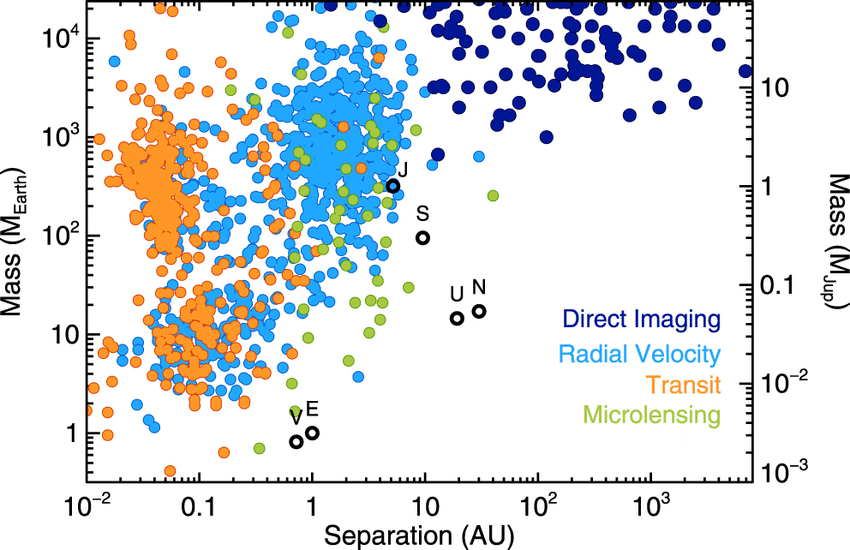
\includegraphics[width=0.8\textwidth]{Exoplanet Demographic Techniques.png}
    \caption{Demographics of exoplanets colored by detection techniques. Credit: Bowler, 2016.}
    \label{fig:techniques}
\end{figure}


\begin{enumerate}
    \item Explain the RV exoplanet detection method in your own words (3-4 sentences).
    \item Explain the transit exoplanet detection method in your own words (3-4 sentences).
    \item Figure \ref{fig:techniques} is a plot of the masses of discovered exoplanets versus their distance from their host stars, colored by the detection method that was used to discover them. Let's think about why certain methods may be biased towards detecting certain types of planets.
    \begin{enumerate}
        \item Using what you learned in this lab, explain why planets detected with the transit technique are (a) primarily massive and (b) close to their host stars. % Massive -> large radius
        \item Using this same plot, we see that we can detect planets using the radial velocity method out to larger separations.
        \begin{enumerate}
            \item Why are we able to use the RV method to detect planets further away from their hosts than the transit method? % Less geometric bias
            \item Why can't we detect small planets far away from their stars using the RV method? % Less ability to tug
        \end{enumerate}
    \end{enumerate}
    \item Based on what you know about the sensitivities of various detection methods, do you think the region that is devoid of objects is a real characteristic of the population of exoplanets or a selection effect? Explain.
    \item Research the Direct Imaging technique (\url{https://en.wikipedia.org/wiki/Methods_of_detecting_exoplanets#Direct_imaging}) and briefly explain how it works.  Why is Direct Imaging biased towards massive planets far from their hosts?
    \item For each of the following fictional scenarios, which detection method would you choose and why? Justify in one sentence.
    \begin{enumerate}
        \item a small rocky, close-in planet in an edge-on system % Transit
        \item a high mass planet moderately far from its host star on a slightly inclined orbit % RV
        \item a very big, bright planet very far out from the star in a face-on system % Direct imaging
    \end{enumerate}
    \item The \textit{Kepler} mission launched in 2009. How has our understanding of the exoplanet population changed since then?
   
\end{enumerate}

\section{Conclusion}
\begin{enumerate}
    \item What did you like or dislike about this lab?
    \item Any feedback/suggestions?
    \item Any remaining questions?
\end{enumerate}

\end{document}